\documentclass[preview,convert={outext=.svg,command=\unexpanded{pdf2svg \infile\space\outfile}},multi=false]{standalone}[2012/04/13]
\usepackage{tikz}
\usetikzlibrary{arrows, calc}
\usepackage{amsmath}

%% common idioms for diagrams
\def\Hask{\mathsf{Hask}}
\def\Id{\mathsf{Id}}
\def\T{\mathsf{T}}
\def\id{\mathsf{id}}



\begin{document}
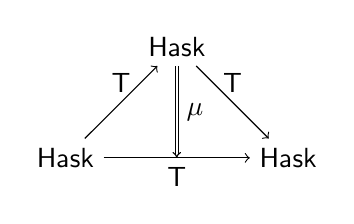
\begin{tikzpicture}[node distance=2cm, auto, baseline=(mu.base)]
  \node (H1) {$\Hask$};
  \node (H2) [above right of= H1] {$\Hask$};
  \node (H3) [below right of= H2] {$\Hask$};
  \draw[->] (H1) to node (t) [above] {$\T$} (H2);
  \draw[->] (H2) to node [above] {$\T$} (H3);
  \draw[->] (H1) to node [below] (t2) {$\T$} (H3);
  \draw[->, double, -implies] (H2) to node (mu)  [right] {$\mu$} (t2); % double arrow needs to be shorter. how do we factor that out?
\end{tikzpicture}
\end{document}
